\documentclass{article}
\usepackage[margin = 1in]{geometry}
\usepackage{graphicx}
\usepackage{amsmath}
\usepackage{amssymb}
\usepackage{bm}
\usepackage{tcolorbox}
\usepackage{latex-rmd}
\newcommand{\E}{\mathrm{E}}
\newcommand{\Log}{\log}
\renewcommand{\log}{\:\mathrm{log}\:}
\renewcommand\thesubsection{\thesection.\alph{subsection}}
\setlength{\parindent}{0em}
\setlength{\parskip}{1em}

\title{Advanced Macroeconometrics - Assignment 2}
\author{Miriam Frauenlob, Elisabeth Fidrmuc, Tim Koenders }
\date{May 2023}

\begin{document}

\maketitle

\vspace{2em}

\begin{tcolorbox}
\centering \itshape The executable code that was used in compiling the assignment is available on GitHub at \href{https://github.com/TimKoenders/macrometrics2}{https://github.com/TimKoenders/macrometrics2}.
\end{tcolorbox}

\newpage


\section*{Question 1}

\begin{Shaded}
\begin{Highlighting}[]
\NormalTok{knitr}\SpecialCharTok{::}\NormalTok{opts\_chunk}\SpecialCharTok{$}\FunctionTok{set}\NormalTok{(}\AttributeTok{fig.width=}\DecValTok{12}\NormalTok{, }\AttributeTok{fig.height=}\DecValTok{8}\NormalTok{, }\AttributeTok{fig\_path=}\StringTok{\textquotesingle{}figures/\textquotesingle{}}\NormalTok{,}\AttributeTok{echo=}\ConstantTok{TRUE}\NormalTok{, }\AttributeTok{warning=}\ConstantTok{FALSE}\NormalTok{, }\AttributeTok{message=}\ConstantTok{FALSE}\NormalTok{)}


\CommentTok{\# Define parameters}
\NormalTok{mu }\OtherTok{\textless{}{-}} \DecValTok{5}
\NormalTok{sigma }\OtherTok{\textless{}{-}} \DecValTok{9}
\NormalTok{n }\OtherTok{\textless{}{-}} \DecValTok{100}

\CommentTok{\# Generate data}
\NormalTok{x }\OtherTok{\textless{}{-}} \FunctionTok{rnorm}\NormalTok{(n, }\AttributeTok{mean =}\NormalTok{ mu, }\AttributeTok{sd =}\NormalTok{ sigma)}

\CommentTok{\# Compute estimates of the mean with the first 1, ..., n draws}
\NormalTok{estimates }\OtherTok{\textless{}{-}} \FunctionTok{cumsum}\NormalTok{(x) }\SpecialCharTok{/} \FunctionTok{seq\_along}\NormalTok{(x)}

\CommentTok{\# Plot estimates}
\FunctionTok{plot}\NormalTok{(estimates, }\AttributeTok{type =} \StringTok{"l"}\NormalTok{, }\AttributeTok{col =} \StringTok{"blue"}\NormalTok{, }\AttributeTok{xlab =} \StringTok{"Sample size"}\NormalTok{, }\AttributeTok{ylab =} \StringTok{"Estimate of the mean"}\NormalTok{)}

\CommentTok{\# Add true mean as a horizontal line}
\FunctionTok{abline}\NormalTok{(}\AttributeTok{h =}\NormalTok{ mu, }\AttributeTok{col =} \StringTok{"red"}\NormalTok{)}
\end{Highlighting}
\end{Shaded}

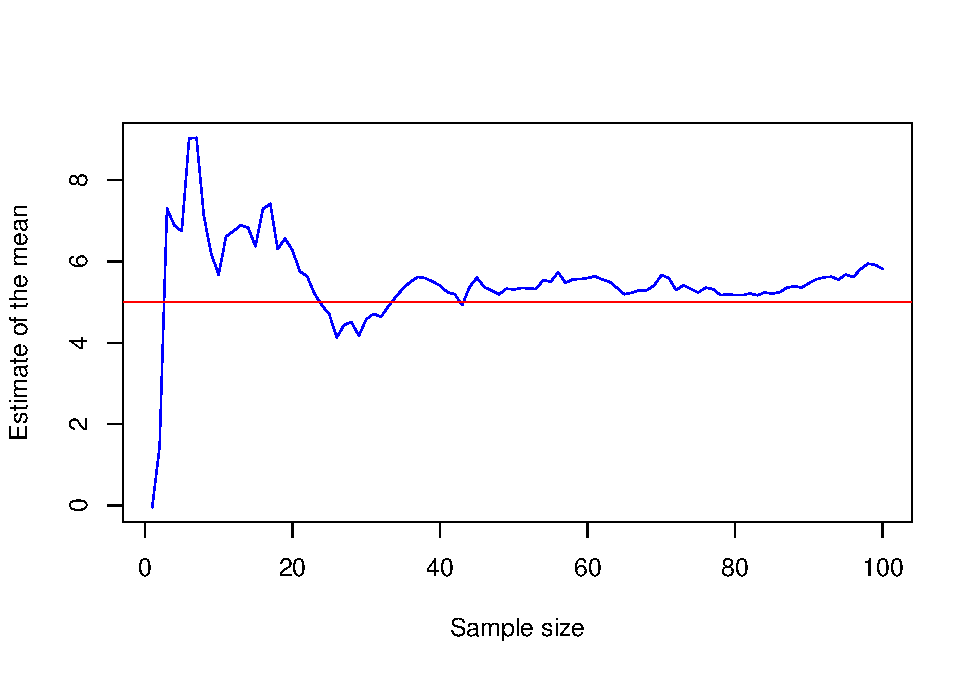
\includegraphics{RMarkdown_files/figure-latex/global_options2-1.pdf}

The plot highlights the law of large numbers in action, where increasing
the sample size results in estimates of the mean that converge to the
true mean. While initial estimates may deviate from the true mean, as
the sample size increases, the estimates become more stable and approach
the true mean with greater precision.

\newpage


\begin{Shaded}
\begin{Highlighting}[]
\NormalTok{knitr}\SpecialCharTok{::}\NormalTok{opts\_chunk}\SpecialCharTok{$}\FunctionTok{set}\NormalTok{(}\AttributeTok{fig.width=}\DecValTok{12}\NormalTok{, }\AttributeTok{fig.height=}\DecValTok{8}\NormalTok{, }\AttributeTok{fig\_path=}\StringTok{\textquotesingle{}figures/\textquotesingle{}}\NormalTok{,}\AttributeTok{echo=}\ConstantTok{TRUE}\NormalTok{, }\AttributeTok{warning=}\ConstantTok{FALSE}\NormalTok{, }\AttributeTok{message=}\ConstantTok{FALSE}\NormalTok{)}

\CommentTok{\# Define parameters}
\NormalTok{mu }\OtherTok{\textless{}{-}} \DecValTok{0}
\NormalTok{sigma }\OtherTok{\textless{}{-}} \DecValTok{1}
\NormalTok{n }\OtherTok{\textless{}{-}} \DecValTok{1000}

\CommentTok{\# Generate two random samples from a standard normal distribution}
\NormalTok{x }\OtherTok{\textless{}{-}} \FunctionTok{rnorm}\NormalTok{(n, }\AttributeTok{mean =}\NormalTok{ mu, }\AttributeTok{sd =}\NormalTok{ sigma)}
\NormalTok{y }\OtherTok{\textless{}{-}} \FunctionTok{rnorm}\NormalTok{(n, }\AttributeTok{mean =}\NormalTok{ mu, }\AttributeTok{sd =}\NormalTok{ sigma)}

\CommentTok{\# Convert the standard normal samples to a Cauchy distribution with scale one}
\NormalTok{z }\OtherTok{\textless{}{-}}\NormalTok{ x }\SpecialCharTok{/}\NormalTok{ y}

\CommentTok{\# Compute estimates of the mean with the first 1, ..., n draws}
\NormalTok{estimates }\OtherTok{\textless{}{-}} \FunctionTok{cumsum}\NormalTok{(z) }\SpecialCharTok{/} \FunctionTok{seq\_along}\NormalTok{(z)}

\CommentTok{\# Plot estimates}
\FunctionTok{plot}\NormalTok{(estimates, }\AttributeTok{type =} \StringTok{"l"}\NormalTok{, }\AttributeTok{col =} \StringTok{"blue"}\NormalTok{, }\AttributeTok{xlab =} \StringTok{"Sample size"}\NormalTok{, }\AttributeTok{ylab =} \StringTok{"Estimate of the mean"}\NormalTok{)}

\CommentTok{\# Add true mean as a horizontal line}
\FunctionTok{abline}\NormalTok{(}\AttributeTok{h =}\NormalTok{ mu, }\AttributeTok{col =} \StringTok{"red"}\NormalTok{)}
\end{Highlighting}
\end{Shaded}

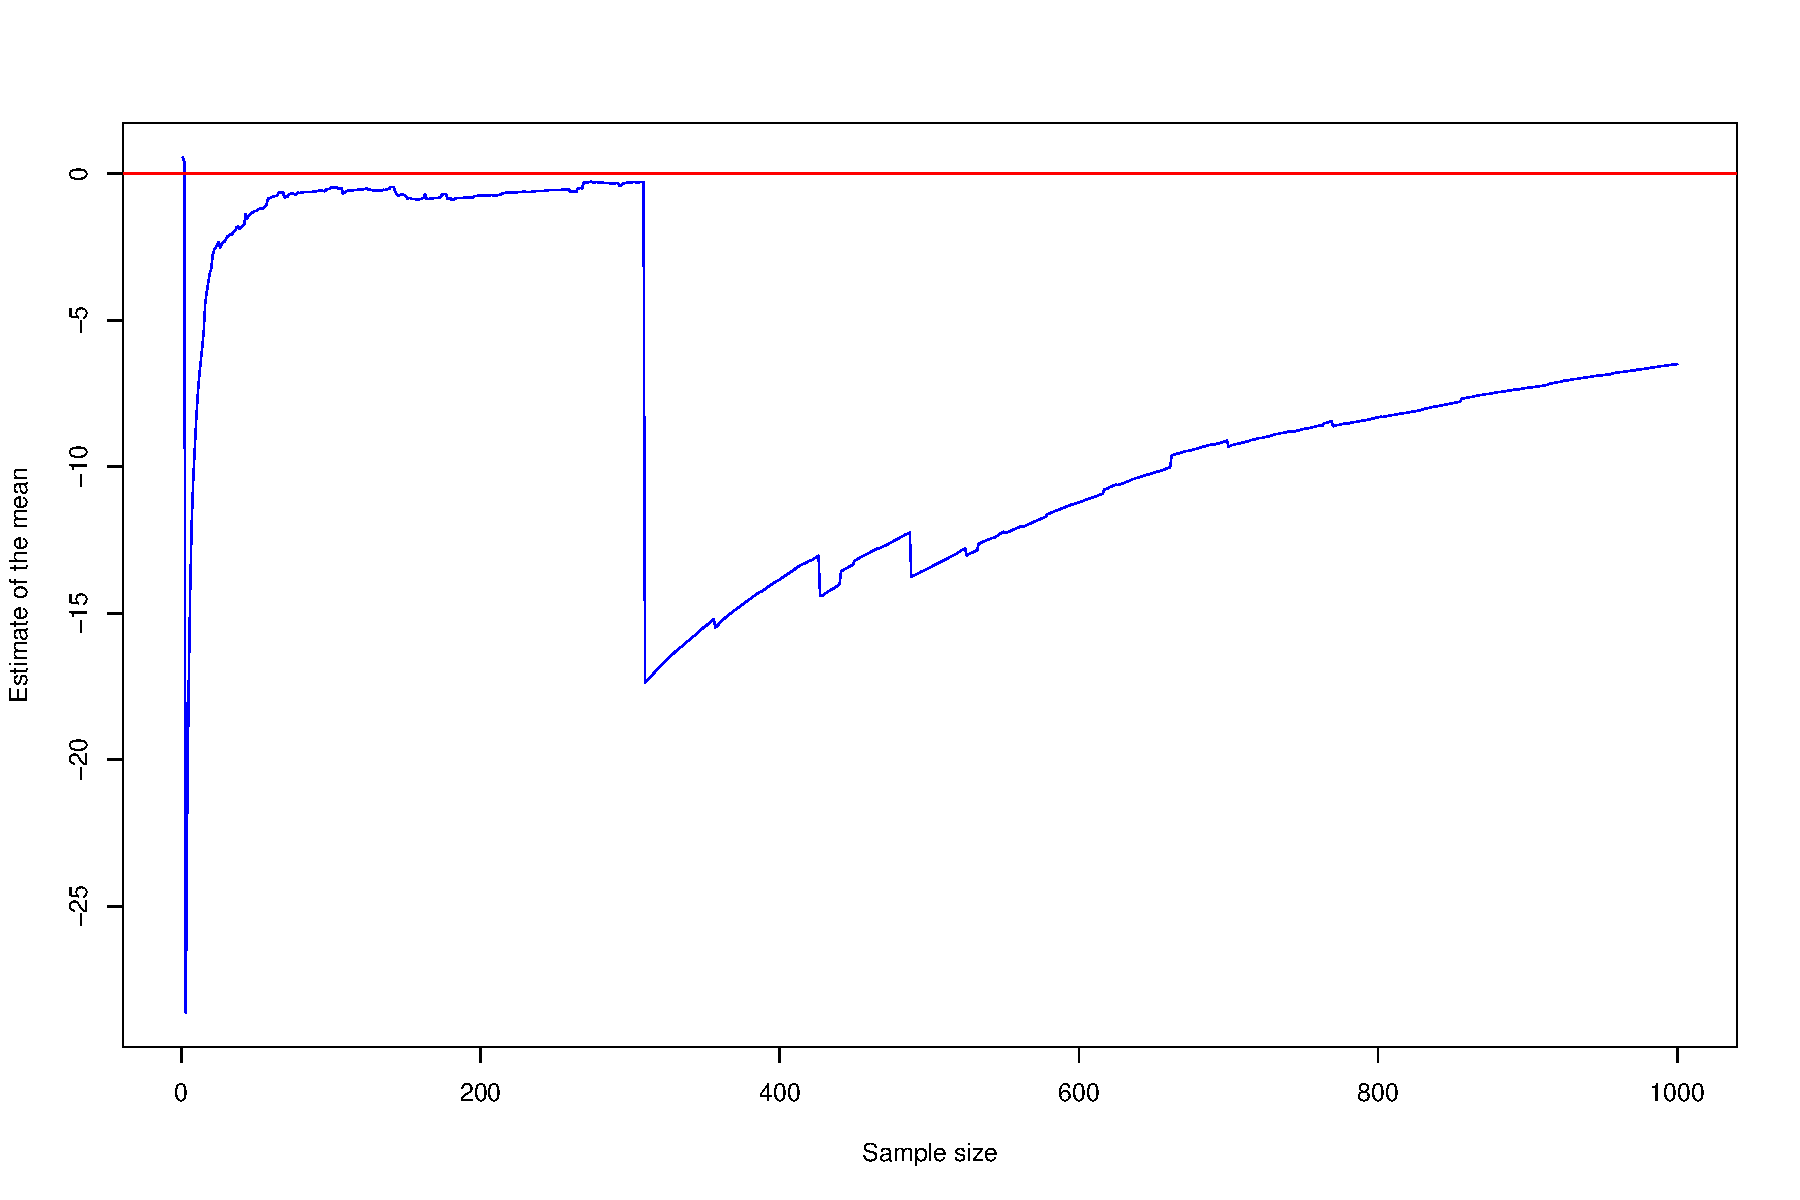
\includegraphics{RMarkdown_files/figure-latex/global_options3-1.pdf}

The plot generated by the code shows the estimates of the mean of a
Cauchy distribution with increasing sample sizes. The blue line
represents the estimated mean, computed as the cumulative sum of the
ratio of two random samples from a standard normal distribution
(converted to a Cauchy distribution), divided by the sample size. The
red line represents the true mean, which is zero in this case.The Cauchy
distribution does not have a well-defined mean and variance, as its
probability density function has ``heavy tails'' that extend to infinity
in both directions. This means that the distribution does not converge
to a particular value as the sample size increases.

\section*{Question 2}

\newpage


\section*{Question 3}

\begin{Shaded}
\begin{Highlighting}[]
\NormalTok{knitr}\SpecialCharTok{::}\NormalTok{opts\_chunk}\SpecialCharTok{$}\FunctionTok{set}\NormalTok{(}\AttributeTok{fig.width=}\DecValTok{12}\NormalTok{, }\AttributeTok{fig.height=}\DecValTok{8}\NormalTok{, }\AttributeTok{fig\_path=}\StringTok{\textquotesingle{}figures/\textquotesingle{}}\NormalTok{,}\AttributeTok{echo=}\ConstantTok{TRUE}\NormalTok{, }\AttributeTok{warning=}\ConstantTok{FALSE}\NormalTok{, }\AttributeTok{message=}\ConstantTok{FALSE}\NormalTok{)}

\CommentTok{\# Question 3}

\NormalTok{simulate\_data }\OtherTok{\textless{}{-}} \ControlFlowTok{function}\NormalTok{(n, k, alpha, beta, sigma) \{}
\NormalTok{  X }\OtherTok{\textless{}{-}} \FunctionTok{matrix}\NormalTok{(}\FunctionTok{rnorm}\NormalTok{(n }\SpecialCharTok{*}\NormalTok{ k, }\AttributeTok{mean =} \DecValTok{0}\NormalTok{, }\AttributeTok{sd =} \DecValTok{1}\NormalTok{), n, k)}
\NormalTok{  epsilon }\OtherTok{\textless{}{-}} \FunctionTok{rnorm}\NormalTok{(n, }\AttributeTok{mean =} \DecValTok{0}\NormalTok{, }\AttributeTok{sd =}\NormalTok{ sigma)}
\NormalTok{  y }\OtherTok{\textless{}{-}}\NormalTok{ alpha }\SpecialCharTok{+}\NormalTok{ X }\SpecialCharTok{\%*\%}\NormalTok{ beta }\SpecialCharTok{+}\NormalTok{ epsilon}
  \FunctionTok{return}\NormalTok{(}\FunctionTok{list}\NormalTok{(}\AttributeTok{X =}\NormalTok{ X, }\AttributeTok{y =}\NormalTok{ y))}
\NormalTok{\}}
\end{Highlighting}
\end{Shaded}

Question 3

\begin{Shaded}
\begin{Highlighting}[]
\NormalTok{knitr}\SpecialCharTok{::}\NormalTok{opts\_chunk}\SpecialCharTok{$}\FunctionTok{set}\NormalTok{(}\AttributeTok{fig.width=}\DecValTok{12}\NormalTok{, }\AttributeTok{fig.height=}\DecValTok{8}\NormalTok{, }\AttributeTok{fig\_path=}\StringTok{\textquotesingle{}figures/\textquotesingle{}}\NormalTok{,}\AttributeTok{echo=}\ConstantTok{TRUE}\NormalTok{, }\AttributeTok{warning=}\ConstantTok{FALSE}\NormalTok{, }\AttributeTok{message=}\ConstantTok{FALSE}\NormalTok{)}

\FunctionTok{set.seed}\NormalTok{(}\DecValTok{123}\NormalTok{)}

\CommentTok{\# Creating function}
\NormalTok{sim\_linear\_model\_1 }\OtherTok{\textless{}{-}} \ControlFlowTok{function}\NormalTok{(n, k, alpha, beta, sigma) \{}
\NormalTok{  X }\OtherTok{\textless{}{-}} \FunctionTok{matrix}\NormalTok{(}\FunctionTok{rnorm}\NormalTok{(n }\SpecialCharTok{*}\NormalTok{ k, }\AttributeTok{mean =} \DecValTok{0}\NormalTok{, }\AttributeTok{sd =} \DecValTok{1}\NormalTok{), n, k)}
\NormalTok{  x }\OtherTok{\textless{}{-}}\NormalTok{ X[,}\DecValTok{1}\NormalTok{]}
\NormalTok{  epsilon }\OtherTok{\textless{}{-}} \FunctionTok{rnorm}\NormalTok{(n, }\AttributeTok{mean =} \DecValTok{0}\NormalTok{, }\AttributeTok{sd =}\NormalTok{ sigma)}
\NormalTok{  y }\OtherTok{\textless{}{-}}\NormalTok{ alpha }\SpecialCharTok{+}\NormalTok{ X }\SpecialCharTok{\%*\%}\NormalTok{ beta }\SpecialCharTok{+}\NormalTok{ epsilon}
  \FunctionTok{return}\NormalTok{(}\FunctionTok{list}\NormalTok{(}\AttributeTok{x =}\NormalTok{ x, }\AttributeTok{y =}\NormalTok{ y))}
  
\NormalTok{\}}

\CommentTok{\# Create scatterplot with regression line}
\NormalTok{sim\_data\_1 }\OtherTok{\textless{}{-}} \FunctionTok{sim\_linear\_model\_1}\NormalTok{(}\AttributeTok{n =} \DecValTok{100}\NormalTok{, }\AttributeTok{k =} \DecValTok{1}\NormalTok{, }\AttributeTok{alpha =} \DecValTok{2}\NormalTok{, }\AttributeTok{beta =} \DecValTok{3}\NormalTok{, }\AttributeTok{sigma =} \DecValTok{1}\NormalTok{)}
\FunctionTok{plot}\NormalTok{(sim\_data\_1}\SpecialCharTok{$}\NormalTok{x, sim\_data\_1}\SpecialCharTok{$}\NormalTok{y, }\AttributeTok{xlab =} \StringTok{"x"}\NormalTok{, }\AttributeTok{ylab =} \StringTok{"y"}\NormalTok{)}
\FunctionTok{abline}\NormalTok{(}\FunctionTok{lm}\NormalTok{(y }\SpecialCharTok{\textasciitilde{}}\NormalTok{ x, }\AttributeTok{data =}\NormalTok{ sim\_data\_1), }\AttributeTok{col =} \StringTok{"red"}\NormalTok{)}
\end{Highlighting}
\end{Shaded}

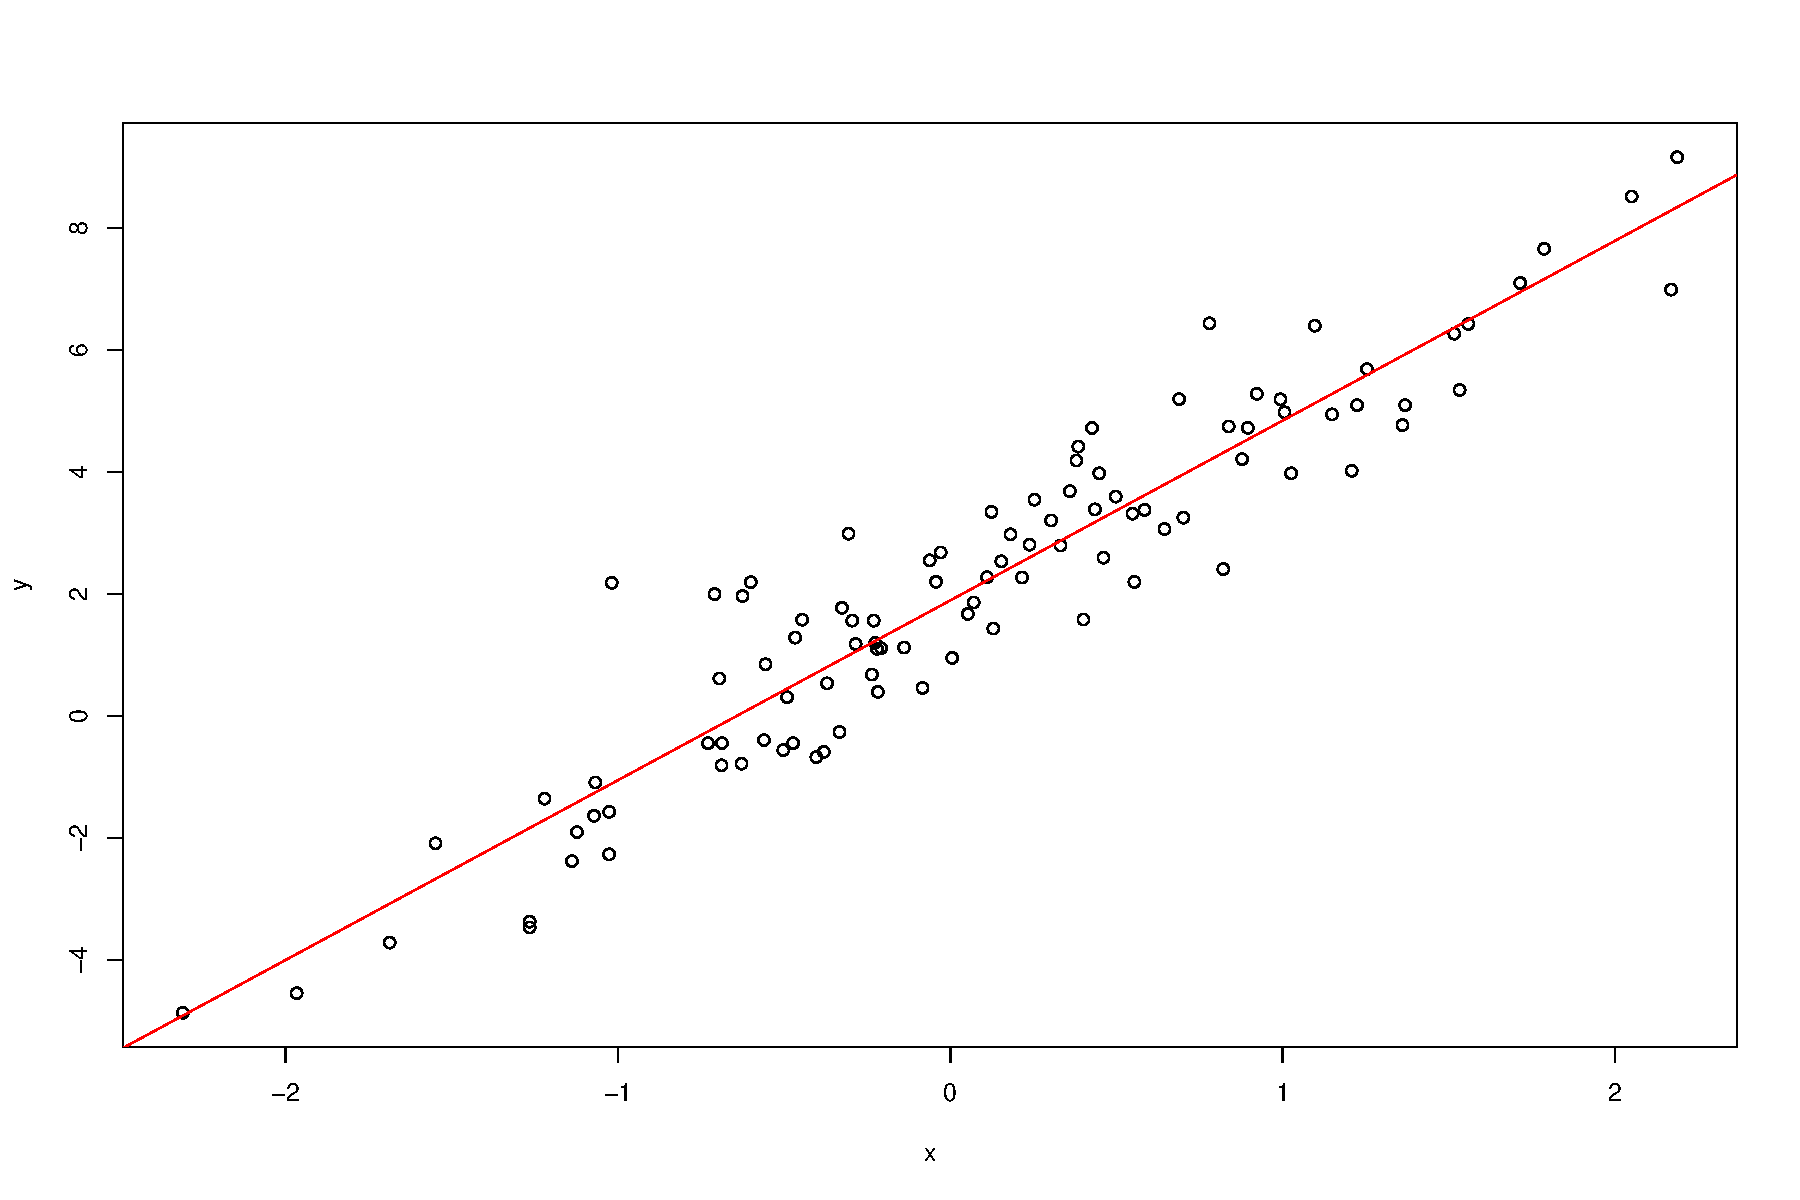
\includegraphics{RMarkdown_files/figure-latex/global_options4-1.pdf}

\begin{Shaded}
\begin{Highlighting}[]
\CommentTok{\# Define numbers of simulations}

\NormalTok{n\_sims }\OtherTok{\textless{}{-}} \DecValTok{1000}

\CommentTok{\# Create an empty vector to store the estimated slope coefficients}
\NormalTok{beta\_lse }\OtherTok{\textless{}{-}} \FunctionTok{numeric}\NormalTok{(n\_sims)}

\CommentTok{\# Loop through the simulations}
\ControlFlowTok{for}\NormalTok{ (i }\ControlFlowTok{in} \DecValTok{1}\SpecialCharTok{:}\NormalTok{n\_sims) \{}
  \CommentTok{\# Simulate the data}
\NormalTok{  sim\_data\_1 }\OtherTok{\textless{}{-}} \FunctionTok{sim\_linear\_model\_1}\NormalTok{(}\AttributeTok{n =} \DecValTok{100}\NormalTok{, }\AttributeTok{k =} \DecValTok{1}\NormalTok{, }\AttributeTok{alpha =} \DecValTok{2}\NormalTok{, }\AttributeTok{beta =} \DecValTok{3}\NormalTok{, }\AttributeTok{sigma =} \DecValTok{1}\NormalTok{)}
  
  \CommentTok{\# Estimate the slope coefficient using linear regression}
\NormalTok{  fit }\OtherTok{\textless{}{-}} \FunctionTok{lm}\NormalTok{(sim\_data\_1}\SpecialCharTok{$}\NormalTok{y }\SpecialCharTok{\textasciitilde{}}\NormalTok{ sim\_data\_1}\SpecialCharTok{$}\NormalTok{x)}
\NormalTok{  beta\_lse[i] }\OtherTok{\textless{}{-}} \FunctionTok{coef}\NormalTok{(fit)[}\DecValTok{2}\NormalTok{]}
\NormalTok{\}}

\CommentTok{\# Creating histogram}
\FunctionTok{hist}\NormalTok{(beta\_lse, }\AttributeTok{main =} \StringTok{"Histogram of Beta Estimates"}\NormalTok{, }\AttributeTok{xlab =} \StringTok{"Beta Estimate"}\NormalTok{)}
\end{Highlighting}
\end{Shaded}

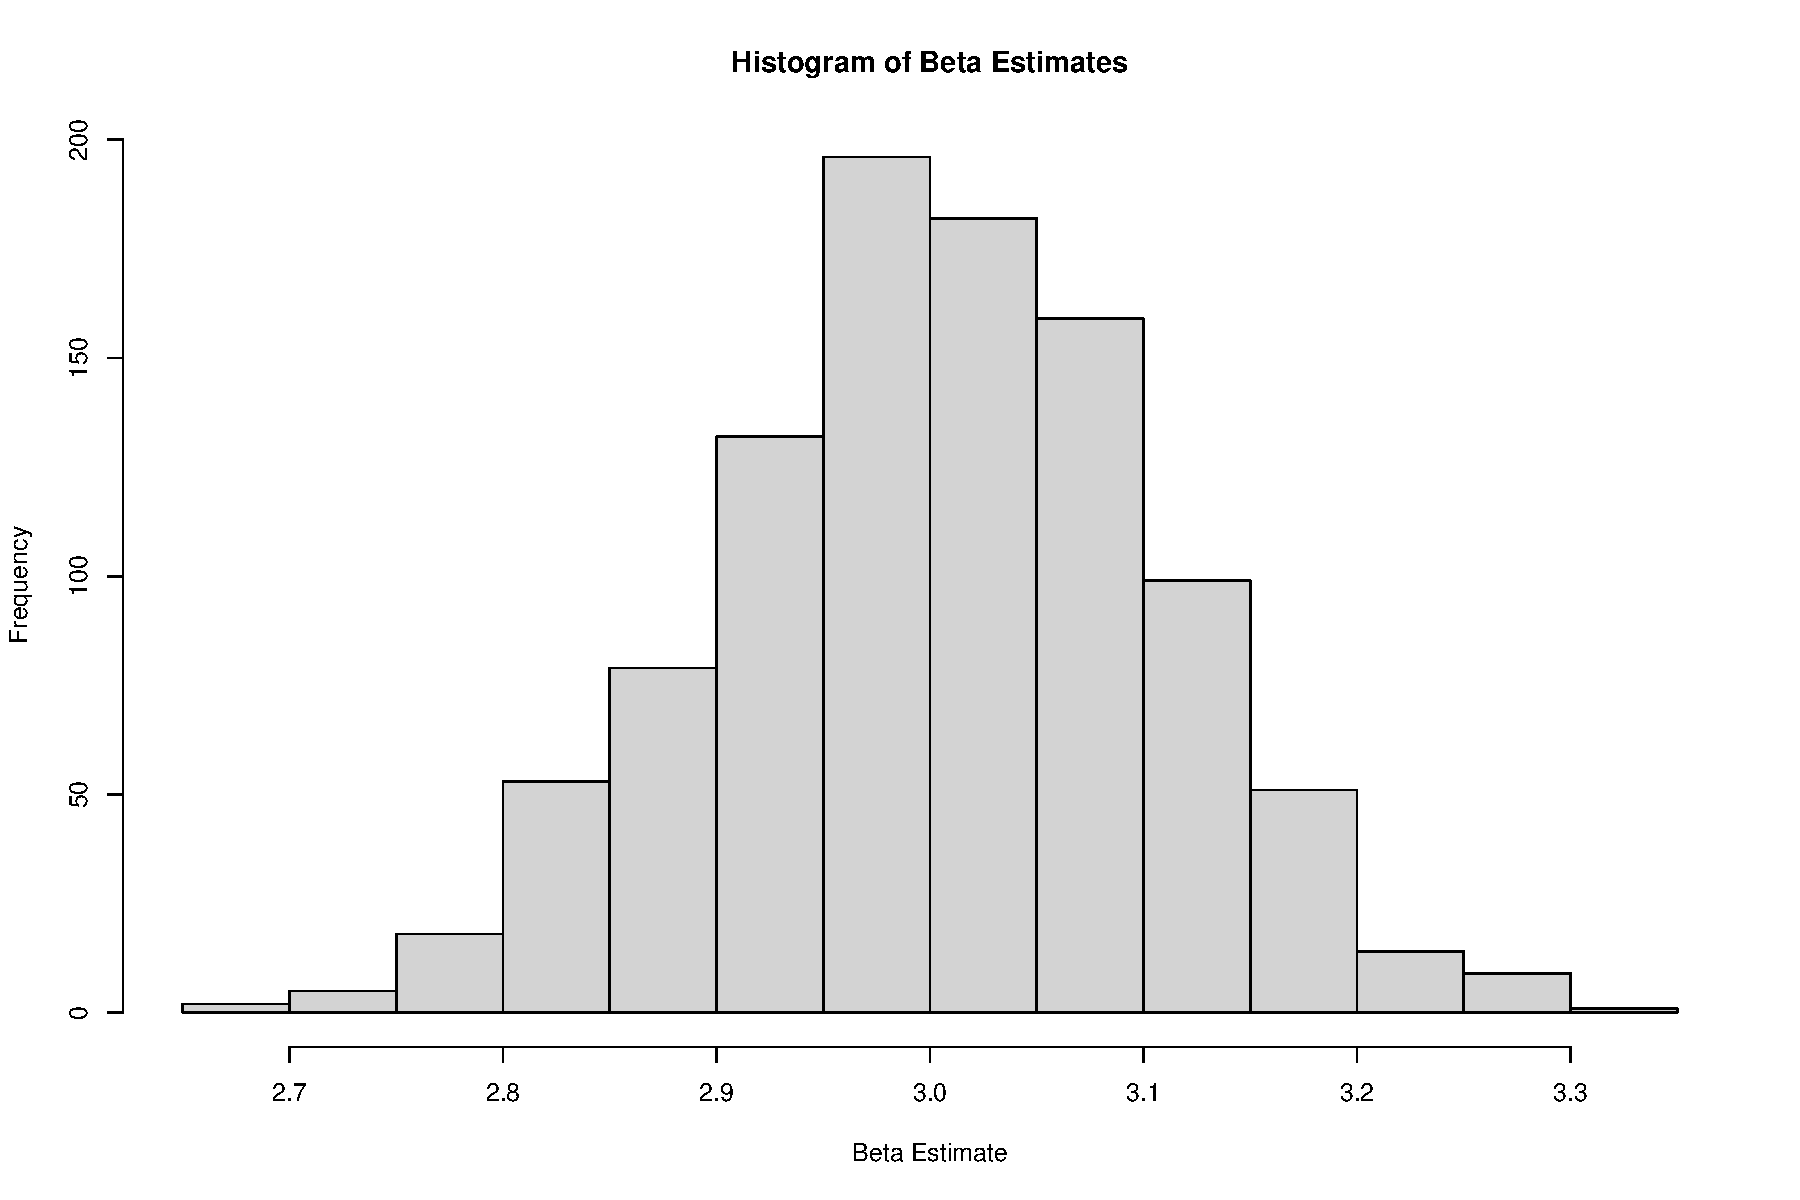
\includegraphics{RMarkdown_files/figure-latex/global_options4-2.pdf} The
approximately normal distribution of the beta\_lse estimates and its
central tendency around the true value of the slope coefficient of 3
suggests that the beta estimate is consistent. This means that as the
number of simulations approaches infinity, the estimates produced by the
estimator will converge to the true population value of the slope
coefficient, and the distribution of estimates will become increasingly
concentrated around the true value.

Latent variables are variables that can only be inferred indirectly from
other observable variables that can be directly observed or measured. In
the given simulation function sim\_linear\_model, the true intercept and
slope coefficient are set to alpha = 2 and beta = 3 respectively, and we
know that the error term has a variance of 1, that is, sigma\^{}2 = 1.
Therefore, the latent values of the model in this case are alpha = 2 and
beta = 3. These values are the true parameters that generate the data,
but they cannot be directly observed or measured. Instead, they are
estimated from the observed data.

One potentially interesting regression to run could be to investigate
the relationship between a person's level of physical activity and their
self-reported levels of happiness. We could use a prior distribution to
specify our beliefs about the coefficient of interest, beta, before
observing any data. For example, we may specify a prior distribution
that assigns higher probability to positive values of beta, based on our
a priori expectation that physical activity is likely to have a positive
effect on happiness. We can then update our beliefs about beta after
observing the data, using Bayes' theorem to obtain the posterior
distribution of beta.

The posterior distribution of beta represents our updated beliefs about
the coefficient after observing the data, taking into account both the
prior distribution and the likelihood of the data given the model. The
posterior distribution can be used to make inferences about the
relationship between physical activity and happiness, such as the
probability that the coefficient of physical activity is positive or
negative, or the range of plausible values for the coefficient.

We will now implement a Bayesian analysis of the relationship between
physical activity and happiness.

\begin{Shaded}
\begin{Highlighting}[]
\NormalTok{knitr}\SpecialCharTok{::}\NormalTok{opts\_chunk}\SpecialCharTok{$}\FunctionTok{set}\NormalTok{(}\AttributeTok{fig.width=}\DecValTok{12}\NormalTok{, }\AttributeTok{fig.height=}\DecValTok{8}\NormalTok{, }\AttributeTok{fig\_path=}\StringTok{\textquotesingle{}figures/\textquotesingle{}}\NormalTok{,}\AttributeTok{echo=}\ConstantTok{TRUE}\NormalTok{, }\AttributeTok{warning=}\ConstantTok{FALSE}\NormalTok{, }\AttributeTok{message=}\ConstantTok{FALSE}\NormalTok{)}

\FunctionTok{library}\NormalTok{(MASS)  }\CommentTok{\# for the mvrnorm function}

\CommentTok{\# Define function to simulate data}
\NormalTok{sim\_linear\_model\_prior }\OtherTok{\textless{}{-}} \ControlFlowTok{function}\NormalTok{(n, k, alpha, beta\_prior\_mean, beta\_prior\_sd, sigma) \{}
\NormalTok{  X }\OtherTok{\textless{}{-}} \FunctionTok{matrix}\NormalTok{(}\FunctionTok{rnorm}\NormalTok{(n }\SpecialCharTok{*}\NormalTok{ k, }\AttributeTok{mean =} \DecValTok{0}\NormalTok{, }\AttributeTok{sd =} \DecValTok{1}\NormalTok{), n, k)}
\NormalTok{  beta }\OtherTok{\textless{}{-}} \FunctionTok{rnorm}\NormalTok{(k, }\AttributeTok{mean =}\NormalTok{ beta\_prior\_mean, }\AttributeTok{sd =}\NormalTok{ beta\_prior\_sd)}
\NormalTok{  epsilon }\OtherTok{\textless{}{-}} \FunctionTok{rnorm}\NormalTok{(n, }\AttributeTok{mean =} \DecValTok{0}\NormalTok{, }\AttributeTok{sd =}\NormalTok{ sigma)}
\NormalTok{  y }\OtherTok{\textless{}{-}}\NormalTok{ alpha }\SpecialCharTok{+}\NormalTok{ X }\SpecialCharTok{\%*\%}\NormalTok{ beta }\SpecialCharTok{+}\NormalTok{ epsilon}
  \FunctionTok{return}\NormalTok{(}\FunctionTok{list}\NormalTok{(}\AttributeTok{X =}\NormalTok{ X, }\AttributeTok{y =}\NormalTok{ y))}
\NormalTok{\}}

\CommentTok{\# Set seed for reproducibility}
\FunctionTok{set.seed}\NormalTok{(}\DecValTok{123}\NormalTok{)}

\CommentTok{\# Set prior parameters mu\_0 and sigma\_0}
\NormalTok{mu\_0 }\OtherTok{\textless{}{-}} \DecValTok{1}
\NormalTok{sigma\_0 }\OtherTok{\textless{}{-}} \DecValTok{2}

\CommentTok{\# Compute posterior for n = 50, 100, and 200}
\ControlFlowTok{for}\NormalTok{ (n }\ControlFlowTok{in} \FunctionTok{c}\NormalTok{(}\DecValTok{50}\NormalTok{, }\DecValTok{100}\NormalTok{, }\DecValTok{200}\NormalTok{)) \{}
  
  \CommentTok{\# Simulate data using sim\_linear\_model\_prior()}
\NormalTok{  k }\OtherTok{\textless{}{-}} \DecValTok{1}
\NormalTok{  alpha }\OtherTok{\textless{}{-}} \DecValTok{0}
\NormalTok{  beta\_prior\_mean }\OtherTok{\textless{}{-}} \DecValTok{0}
\NormalTok{  beta\_prior\_sd }\OtherTok{\textless{}{-}} \DecValTok{1}
\NormalTok{  sigma }\OtherTok{\textless{}{-}} \DecValTok{1}
  
\NormalTok{  sim\_data }\OtherTok{\textless{}{-}} \FunctionTok{sim\_linear\_model\_prior}\NormalTok{(n, k, alpha, beta\_prior\_mean, beta\_prior\_sd, sigma)}
\NormalTok{  X }\OtherTok{\textless{}{-}}\NormalTok{ sim\_data}\SpecialCharTok{$}\NormalTok{X}
\NormalTok{  y }\OtherTok{\textless{}{-}}\NormalTok{ sim\_data}\SpecialCharTok{$}\NormalTok{y}
  
  \CommentTok{\# Compute posterior parameters}
\NormalTok{  sigma\_n }\OtherTok{\textless{}{-}} \FunctionTok{solve}\NormalTok{(sigma\_0}\SpecialCharTok{\^{}}\NormalTok{(}\SpecialCharTok{{-}}\DecValTok{1}\NormalTok{) }\SpecialCharTok{+} \FunctionTok{t}\NormalTok{(X) }\SpecialCharTok{\%*\%}\NormalTok{ X)}
\NormalTok{  mu\_n }\OtherTok{\textless{}{-}}\NormalTok{ sigma\_n }\SpecialCharTok{\%*\%}\NormalTok{ (sigma\_0}\SpecialCharTok{\^{}}\NormalTok{(}\SpecialCharTok{{-}}\DecValTok{1}\NormalTok{) }\SpecialCharTok{*}\NormalTok{ mu\_0 }\SpecialCharTok{+} \FunctionTok{t}\NormalTok{(X) }\SpecialCharTok{\%*\%}\NormalTok{ y)}
  
  \CommentTok{\# Plot posterior density}
\NormalTok{  x\_grid }\OtherTok{\textless{}{-}} \FunctionTok{seq}\NormalTok{(}\SpecialCharTok{{-}}\DecValTok{5}\NormalTok{, }\DecValTok{5}\NormalTok{, }\AttributeTok{length.out =} \DecValTok{1000}\NormalTok{)}
\NormalTok{  post\_dens }\OtherTok{\textless{}{-}} \FunctionTok{dnorm}\NormalTok{(x\_grid, }\AttributeTok{mean =}\NormalTok{ mu\_n, }\AttributeTok{sd =} \FunctionTok{sqrt}\NormalTok{(sigma\_n))}
  \FunctionTok{plot}\NormalTok{(x\_grid, post\_dens, }\AttributeTok{type =} \StringTok{"l"}\NormalTok{, }\AttributeTok{lwd =} \DecValTok{2}\NormalTok{, }\AttributeTok{main =} \FunctionTok{paste0}\NormalTok{(}\StringTok{"Posterior Density (n = "}\NormalTok{, n, }\StringTok{")"}\NormalTok{))}
  
\NormalTok{\}}
\end{Highlighting}
\end{Shaded}

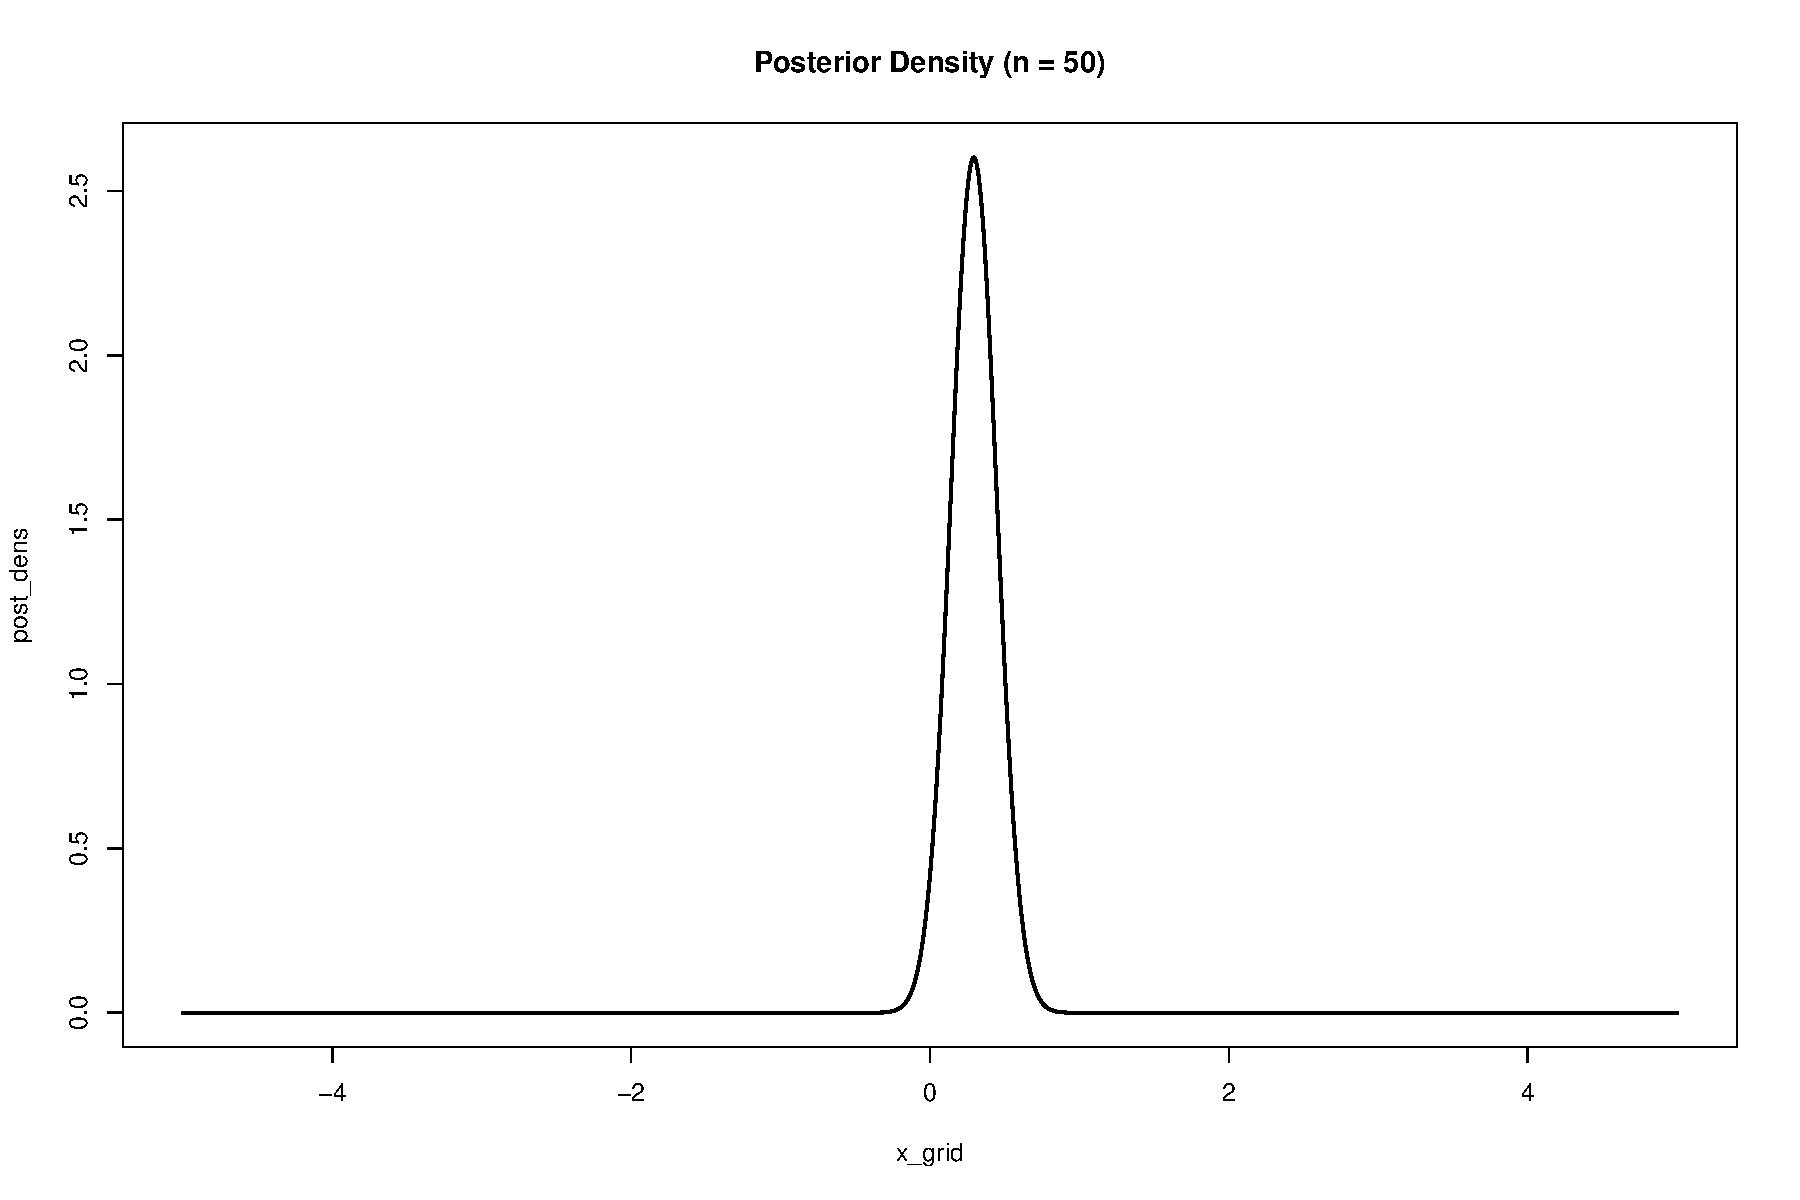
\includegraphics{RMarkdown_files/figure-latex/global_options5-1.pdf}
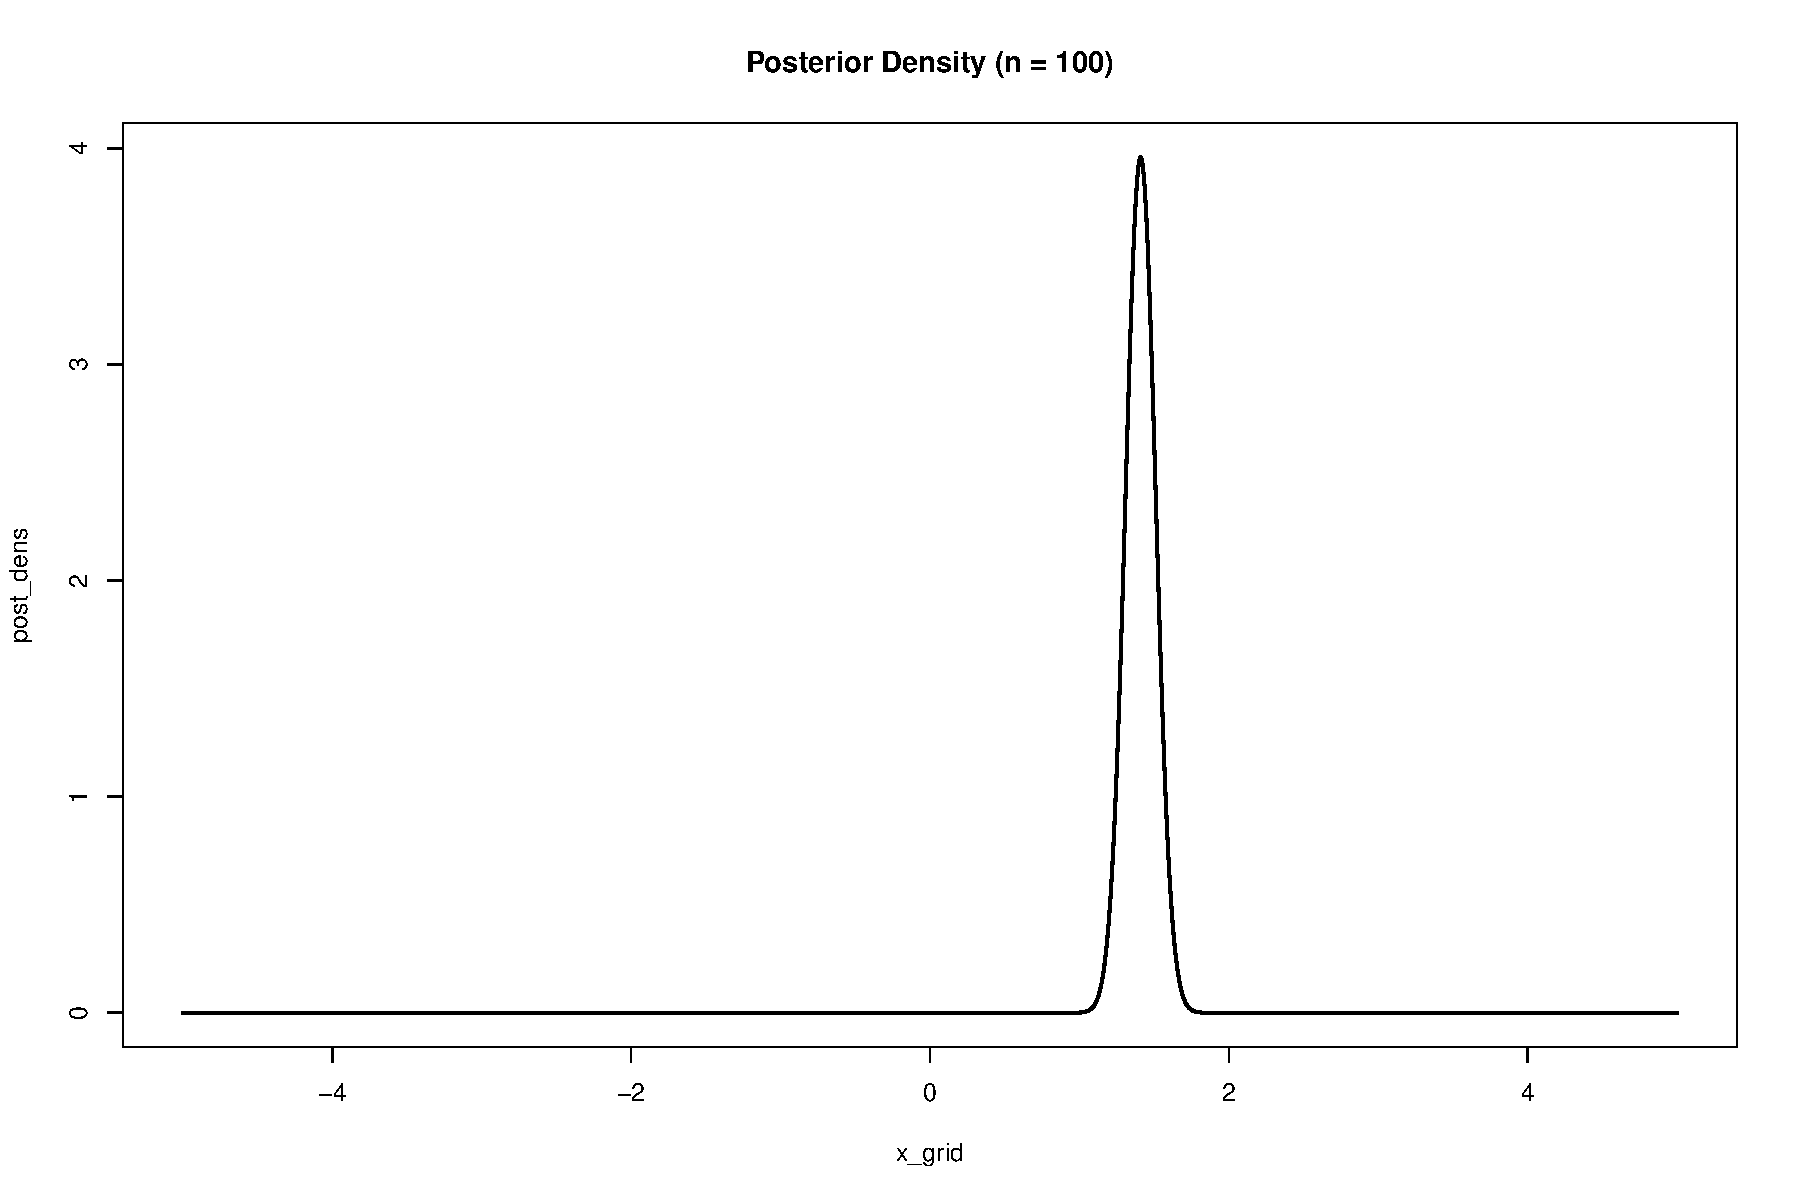
\includegraphics{RMarkdown_files/figure-latex/global_options5-2.pdf}
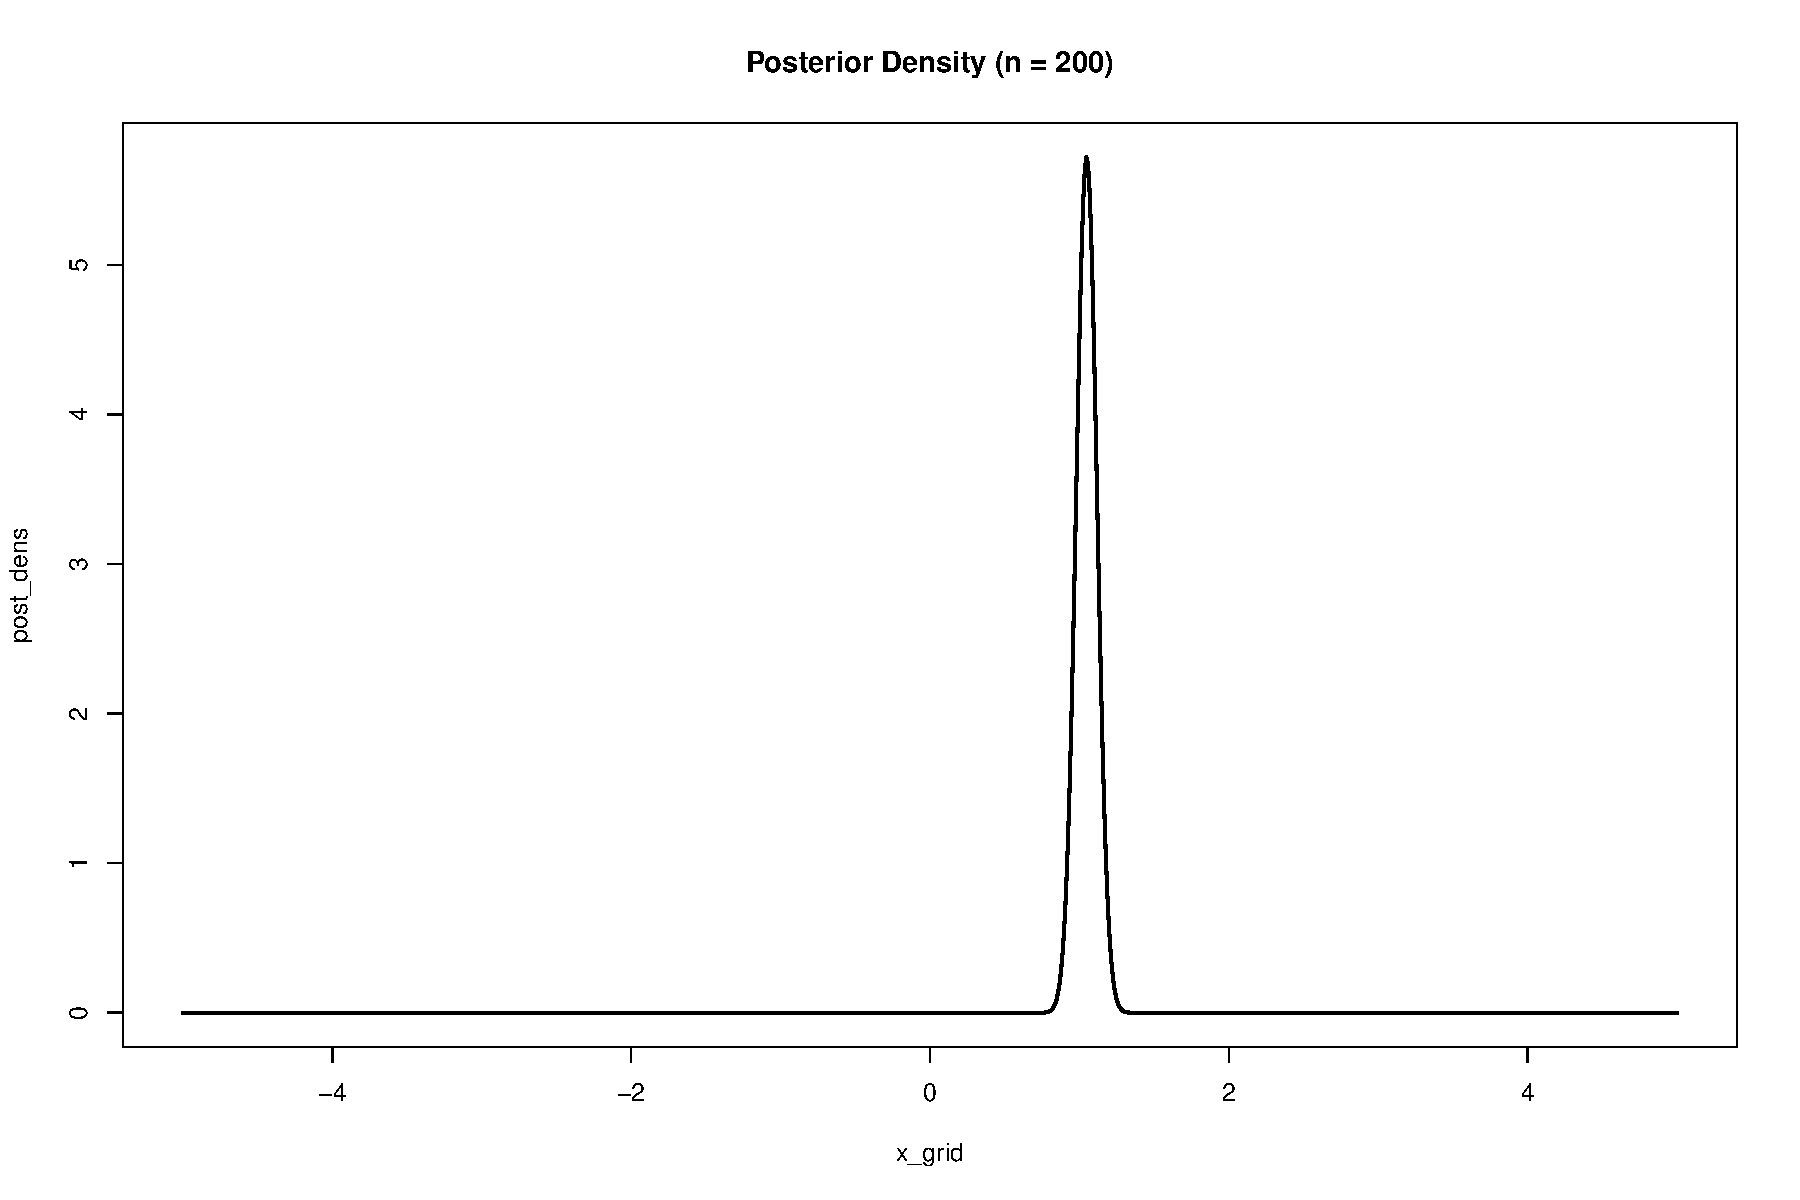
\includegraphics{RMarkdown_files/figure-latex/global_options5-3.pdf}

We are interested in the relationship between a person's level of
physical activity and their self-reported levels of happiness. To
incorporate our prior beliefs about this relationship, we set a positive
prior on the slope coefficient beta. The mean of the prior distribution
is set to 1, indicating that we believe physical activity is likely to
have a positive effect on happiness, while the standard deviation of the
prior distribution is set to 2, indicating that we allow for a wide
range of plausible values for the slope coefficient beta.

The plots of the posterior density, given different sample sizes, show
that, as the sample size increases, the posterior density becomes more
concentrated around the true value of the slope parameters.
Additionally, as the sample size increases, the posterior density
becomes narrower, indicating that the uncertainty in the posterior
estimate decreases.


\end{document}




